\chapter{Theory and Methods}
\begin{comment}

% Questa è la parte che avevo inizialmente scritto io
To investigate the optical jitter affecting a pulsed laser source, it is first essential to establish a clear and simple definition of what jitter is.
\autoref{Sec:Def-Jitter} is dedicated to this purpose, beginning with a basic definition derived from signal theory, zooming in into the topic and introducing some key definitions, as well as an initial example to then end up providing a proper categorization of the sources of jitter.

\autoref{sec:Def-Pulses} provides the reader with the essential background on optical pulses, including key temporal properties and their connection to the spectral domain, with the important mention of the Time-Bandwidth product.
Finally, \autoref{sec:Def-Techniques} offers the theoretical foundation behind the main experimental techniques used in this work, serving as a conceptual bridge between the theory and the measurements discussed in later chapters.



\section{Timing Jitter}
\label{Sec:Def-Jitter}

To better understand what jitter means in the context of optical pulses, we must first give the general definition.

Jitter was originally defined in signal theory as the deviation of the timing instants 
of a sequence of events from their ideal positions in time.
It can affect not only signals that are meant to be rhythmically constant—such as the ticks of a 
clock—but also repetitive or quasi-periodic signals that may include asynchronous events [IEEE Standard \cite{General_IEEE}].

In this thesis, we study jitter in the context of optical pulses, which serve as carriers of timing information
 for our experimental instruments and detectors. Given this focus, the more specific notion of timing jitter is most relevant.
According to the IEEE, timing jitter is defined as the deviation of 
the actual timing instants of a waveform from their ideal temporal positions \cite{General_IEEE}.

We introduce for a better understanding the \autoref{AddAmpl}, where it's shown the timing jitter caused by an additive amplitude noise on the timing signal.
In this image the noisy rising edge of the waveform crosses the detection threshold over a range of reference instants that deviate from the ideal reference position. Throughout this thesis this is the first time that we mention the role of thresholding, and it is not a case that this will happen already at the very beginning like here, especially because it is fundamental to understand that only one threshold crossing will be detected, per single part of the waveform. The only important question is when such event will happen, with respect of the ideal position in time. This is the whole idea behind the study of timing jitter.

\begin{figure}[hbtp]
\centering
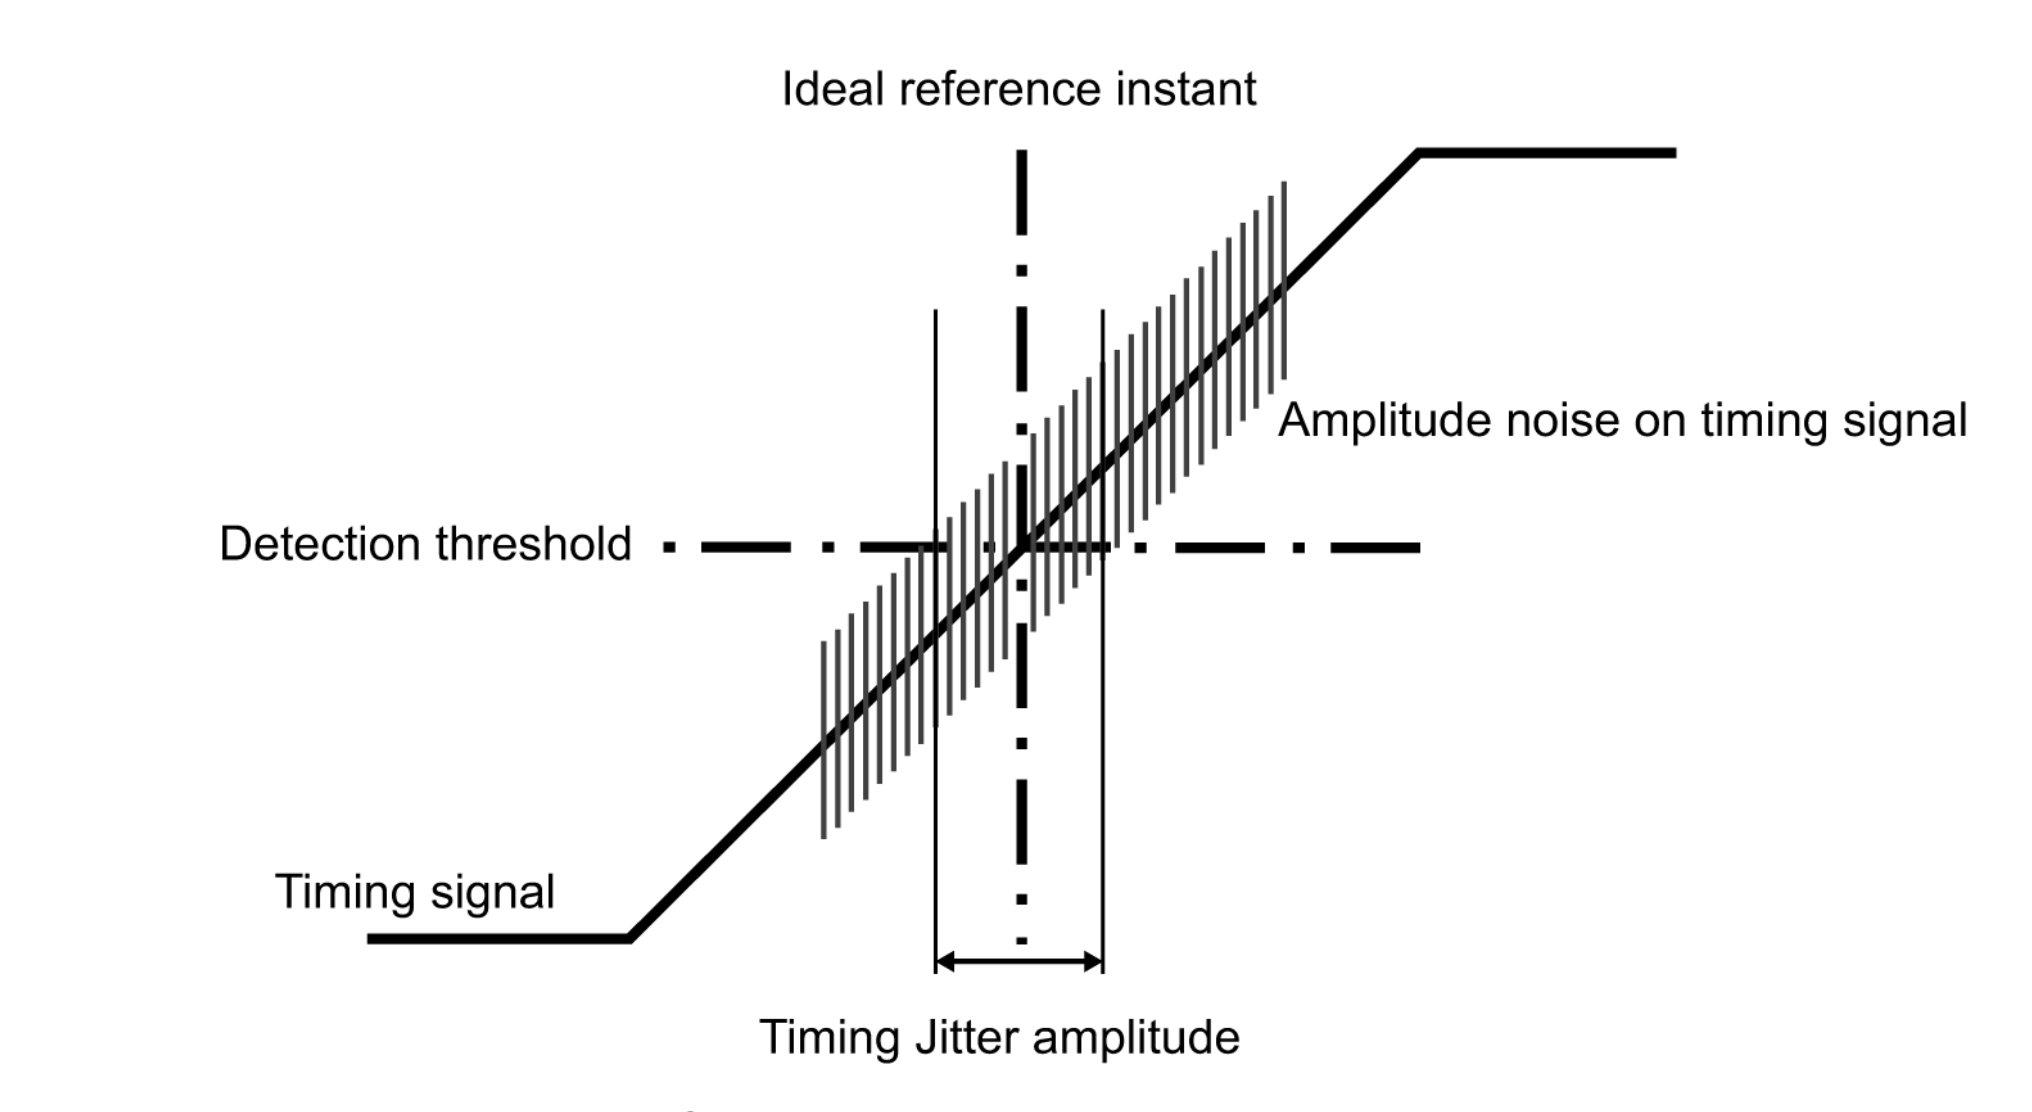
\includegraphics[width=1\textwidth]{AmplitudeAdditiveNoise}
\caption{ Example of timing Jitter induced by an additive amplitude noise \cite{General_IEEE}}
 \label{AddAmpl}
\end{figure} 


\end{comment}

%Questa è la versione ottimizzata una prima volta
To investigate the optical jitter affecting a pulsed laser source, it is first essential to establish a clear and simple definition of what jitter is.  
\autoref{Sec:Def-Jitter} is dedicated to this purpose, beginning with a fundamental definition derived from signal theory, then gradually refining the concept with key terminology and a relevant example. The section concludes by introducing a basic categorization of the main jitter sources.

\autoref{sec:Def-Pulses} provides the reader with the essential background on optical pulses, highlighting their temporal properties and their connection to the spectral domain. Particular attention is given to the Time-Bandwidth product, which plays a central role in later analysis.

Finally, \autoref{sec:Def-Techniques} outlines the theoretical foundations of the experimental techniques employed throughout this work, serving as a conceptual bridge between the physical principles and the measurements presented in the following chapters.

\section{Timing Jitter}
\label{Sec:Def-Jitter}

To understand jitter in the context of optical pulses, we must begin with its general definition.

Jitter was originally introduced in signal theory as the deviation of the timing instants of a sequence of events from their ideal temporal positions. It can affect not only signals designed to be rhythmically constant—such as clock ticks—but also repetitive or quasi-periodic signals, including those with asynchronous components~\cite{General_IEEE}.

In this thesis, we focus on jitter as it appears in optical pulses, which serve as carriers of precise timing information for our instruments and detectors. For this reason, the specific notion of \emph{timing jitter} is most relevant. According to the IEEE, timing jitter is defined as the deviation of the actual timing instants of a waveform from their ideal temporal positions~\cite{General_IEEE}.

To aid understanding, we introduce \autoref{AddAmpl}, which shows an example of timing jitter induced by additive amplitude noise on a signal’s rising edge. In the figure, the noisy waveform crosses the detection threshold over a spread of time instants, deviating from the ideal reference point.

This is the first mention in the thesis of thresholding—a concept that is deliberately introduced early, as it is central to the interpretation of timing jitter. Only one threshold crossing is registered per signal transition; the essential question becomes when this crossing occurs, relative to the ideal time. This forms the core of timing jitter analysis.

\begin{figure}[hbtp]
\centering
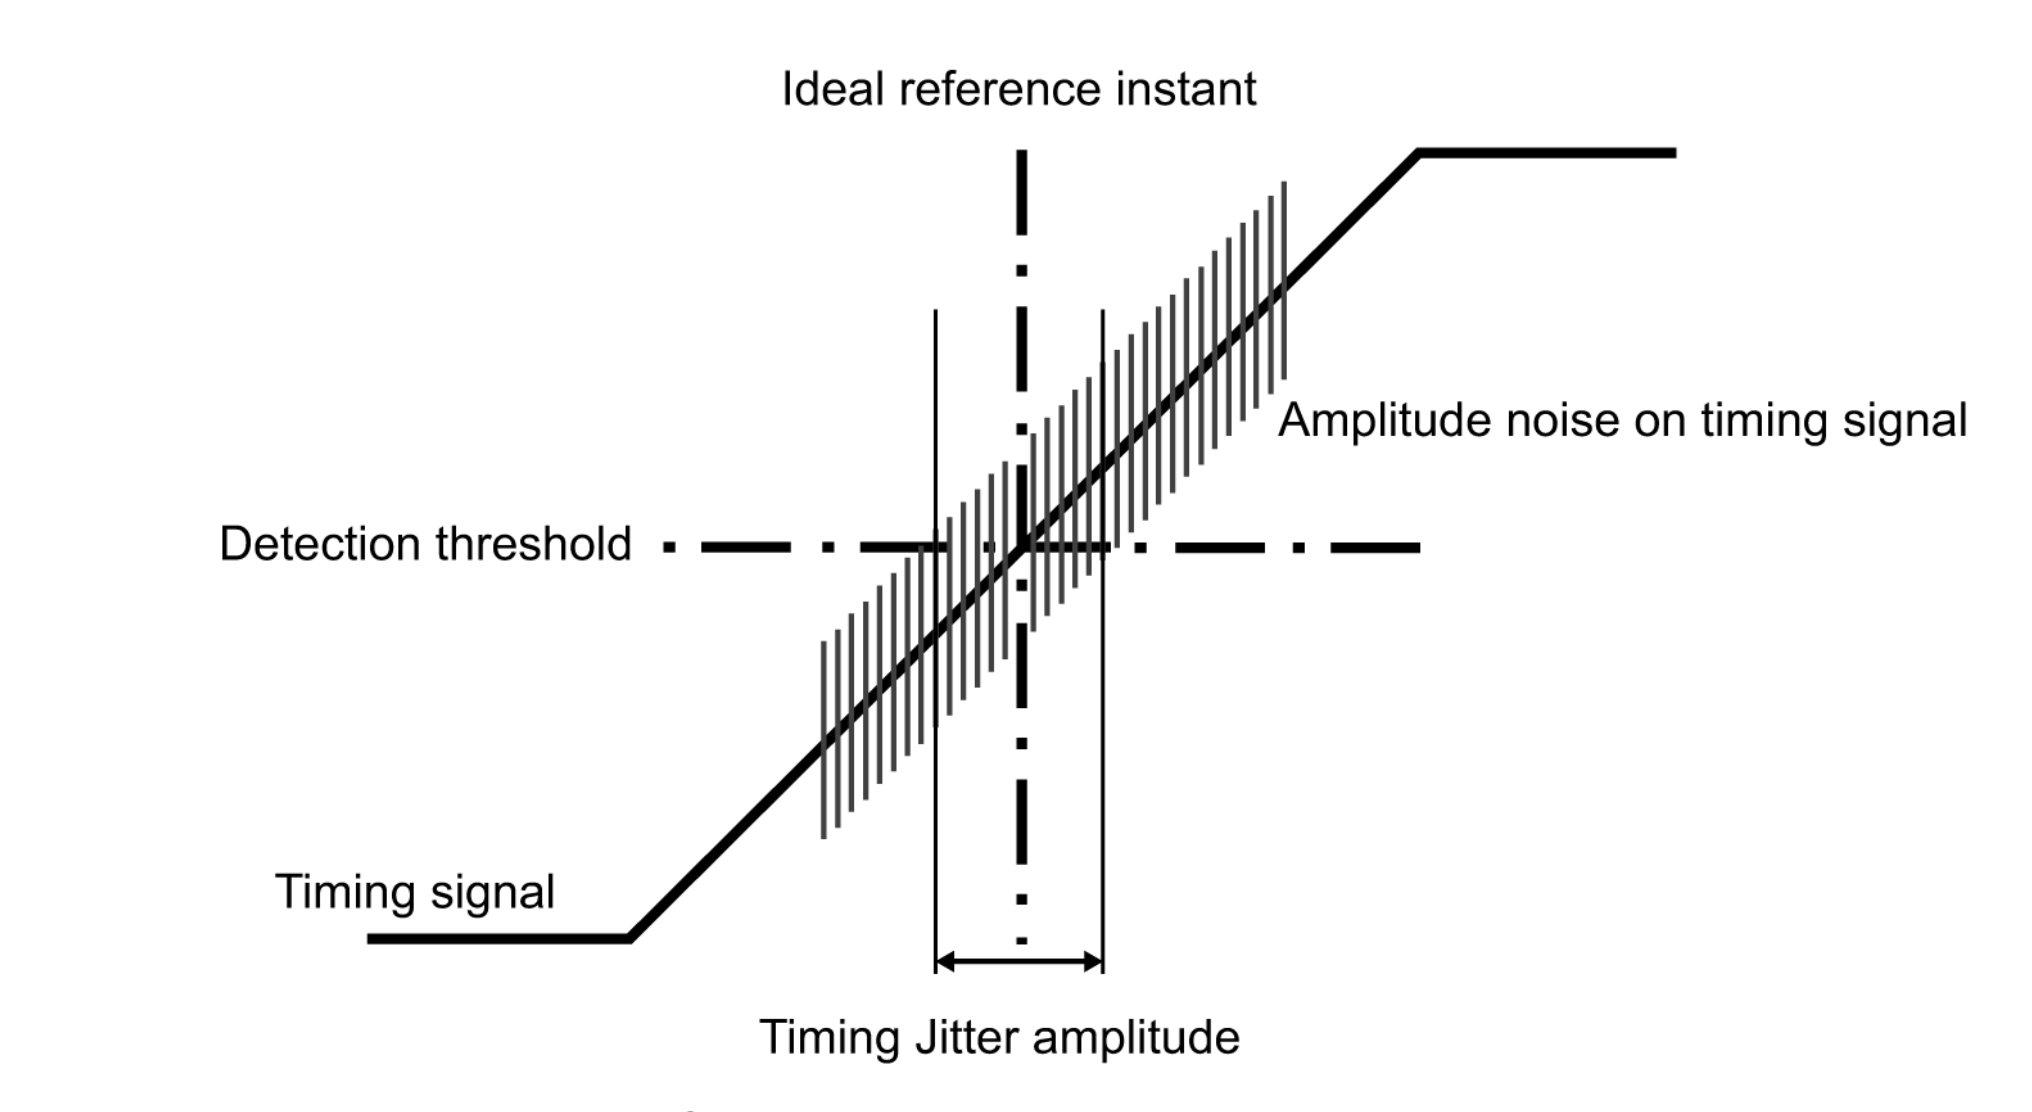
\includegraphics[width=1\textwidth]{AmplitudeAdditiveNoise}
\caption{Example of timing jitter induced by additive amplitude noise~\cite{General_IEEE}.}
\label{AddAmpl}
\end{figure}

%INIZIO DEL SOTTOCAPITOLO CON LA DESCRIZIONE DELLA CATEGORIZZAZIONE DEL TIMING JITTER IN RANDOMICO O DETERMINISTICO
\subsection{Classification of timing jitter sources}

Timing jitter can be broadly classified into two main categories: \emph{deterministic jitter (DJ)} and \emph{random jitter (RJ)}. This distinction is useful to understand the nature of different noise mechanisms and how they combine to affect the precision of a timing signal.

Deterministic jitter arises from predictable, repeatable sources such as crosstalk, power supply noise, or duty cycle distortion. In contrast, random jitter originates from stochastic processes, such as thermal noise or quantum fluctuations in detection, and is inherently unbounded over long timescales.

We identify with the name Random jitter (RJ) all those jitter sources that don't allow successive references to be systematically determined, and this is the reason why the mathematical treatment, just like in Quantum Physics, translates to a statistical framework.
By applying the Central limit theory, RJ can be treated as a mean zero distortion of the waveform, with an underlying gaussian probability density function $f_{RJ}(x)$.

\begin{equation}
f_{RJ}(x) = \frac{1}{\sigma \sqrt{2 \pi }}e^{-\frac{x^2}{2 \sigma ^2}}
\label{eq:RandJitter}
\end{equation}
In this function we can identify x as the random variable that eventually gives contribution to the Total Jitter (TJ), as well as the standard deviation $\sigma$ that defines entirely the features of $f_{RJ}(x)$.

In presence of low contributions in terms of deterministic jitter, Random Jitter can be studied starting from a considerable number of timing errors observed, to which it's possible to draw a statistic and proceed with the analysis.

\autoref{RandomIMG} (a) shows how the pdf $f_{RJ}(x)$ describes the random contribution in terms of jitter to the actual position of the waveform, without forgetting that such random extraction  happens for every rising or falling edge of the waveform independently.

Deterministic Jitter (DJ) on the other hand is a type of jitter that can be 

\begin{figure}[hbtp]
\centering
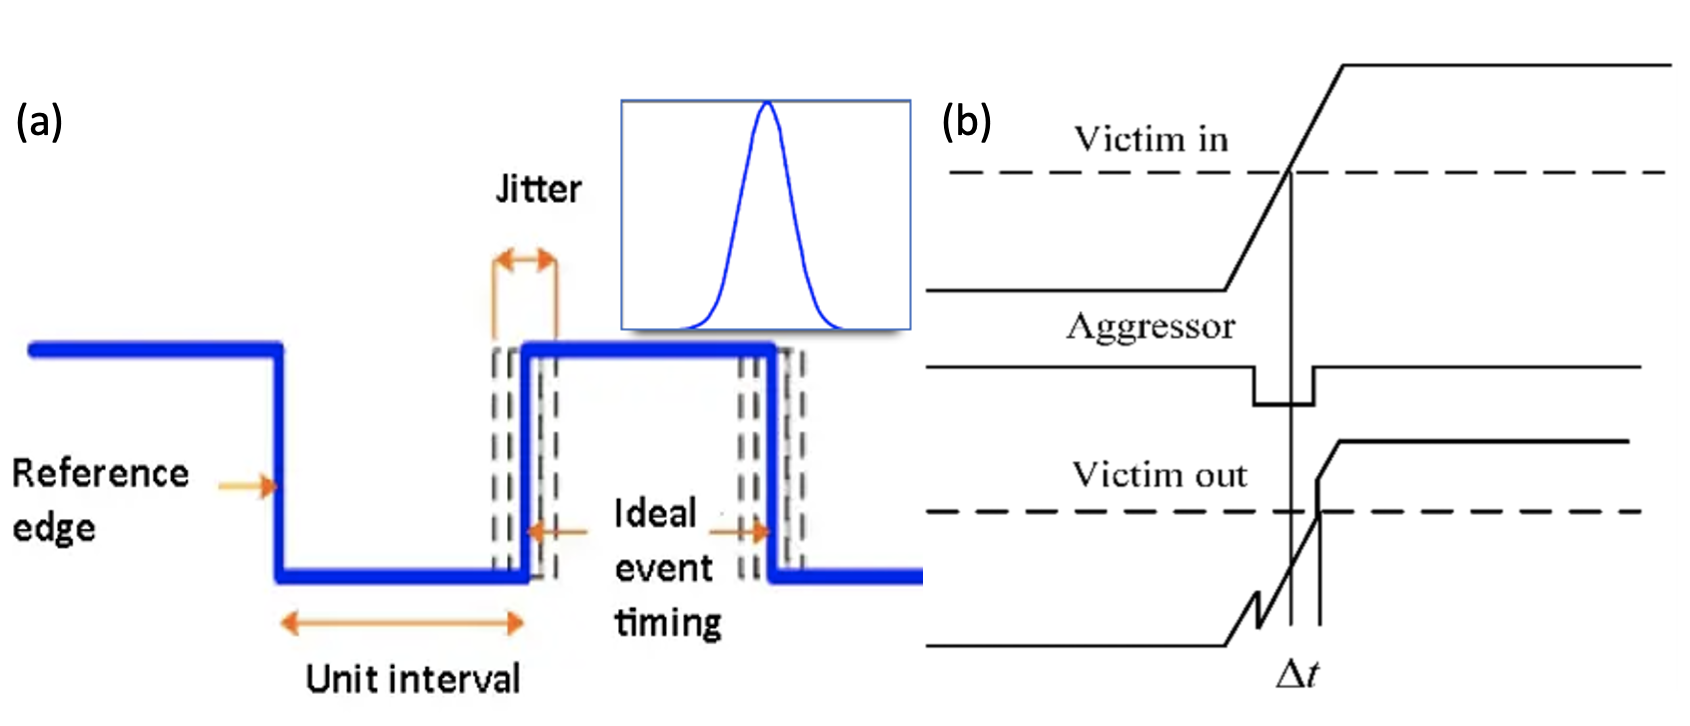
\includegraphics[width=1\textwidth]{RandomCrosstalk}
\caption{(a)Visual representation of the concept of stochastic contribution to timing jitter caused by RJ, here represented with its relative pdf.
(b) Sketch representing the timing jitter caused by an external crosstalk aggressor signal, striking the reference signal and causing the detection event to shift in time because of that.}
\label{RandomIMG}
\end{figure}


\section{Optical pulses}
\label{sec:Def-Pulses}


%Scaletta di cose da dire secondo il nostro caro amico in comune !!!
\begin{comment}
1. Introduction to Optical Pulses
Define what an optical pulse is (brief burst of electromagnetic energy in the optical domain).
Mention the typical time scales involved (fs–ns), depending on the source.
Relate it to your experiment: pulsed laser sources as timing references.
2. Key Temporal Properties
Pulse duration (FWHM): define it and note that it's a crucial timing parameter.
Amplitude and energy: mention intensity profiles, peak power vs. average power.
Repetition rate / period: introduce the temporal spacing between pulses in a mode-locked laser.
3. Temporal and Spectral Domain
Discuss the duality: every pulse has a spectral counterpart.
Present the Fourier transform relationship (not too mathematically, unless your audience expects it).
Emphasize that shorter pulses have broader spectra.
Show how the pulse shape (Gaussian, sech², Lorentzian) affects both time and frequency profiles.
4. Pulse Evolution and Distortion
Briefly describe how optical pulses evolve when propagating through media (e.g., fibers).
Introduce group velocity dispersion (GVD) as the main reason for pulse broadening.
Mention nonlinear effects only if relevant later in your thesis (e.g., self-phase modulation).
5. Time-Bandwidth Product
Define the TBP and explain its role as a measure of pulse quality.
Include TBP values for common shapes: Gaussian (0.44), sech² (0.315), etc.
Explain that TBP sets a fundamental limit: bandwidth and pulse duration cannot both be arbitrarily small.
Optionally, relate to your experiment: estimating the expected pulse duration from spectral width.
\end{comment}



\section{HBT and TCSPC: Measuring and interpreting ps optical jitter}
\label{sec:Def-Techniques}

%Scaletta di cose da dire secondo il nostro caro amico in comune !!!

% ====================== INIZIO SCALETTA SEZIONE TECNICHE SPERIMENTALI ======================
% 1. Second-Order Correlation Function
%    - Introdurre g^{(2)}(τ) come misura statistica delle correlazioni temporali tra eventi di rivelazione fotonica.
%    - Spiegare il significato per diverse sorgenti luminose: luce classica, termica, coerente, singoli fotoni.
%    - Esplicitare la sua forma normalizzata:
%        g^{(2)}(τ) = ⟨I(t) I(t+τ)⟩ / ⟨I(t)⟩^2
%      oppure per rivelazione discreta:
%        g^{(2)}(τ) ∝ N_{12}(τ) / (N_1 ⋅ N_2)
%    - Interpretazione qualitativa:
%        • g^{(2)}(0) < 1 → luce sub-poissoniana (quantistica, antibunching)
%        • g^{(2)}(0) = 1 → luce coerente (Poissoniana)
%        • g^{(2)}(0) > 1 → luce termica (bunched)

% 2. Configurazione HBT
%    - Descrivere lo schema con beam splitter: un impulso ottico diviso su due rivelatori.
%    - Obiettivo: misurare conteggi in coincidenza tra rivelatori.
%    - Evidenziare l'importanza dei ritardi temporali tra eventi.
%    - Limitazioni:
%        • Risoluzione temporale limitata dalla risposta dei rivelatori e dell'elettronica.
%        • Necessaria normalizzazione accurata.

% 3. TCSPC (Time-Correlated Single Photon Counting)
%    - Principio: registrare intervallo temporale tra un trigger (es. sync laser) e rivelazione di un singolo fotone.
%    - Si accumula un istogramma su molti impulsi.
%    - Risultato: profilo temporale della probabilità di rivelazione (convoluto con risposta del sistema).
%    - Perché è così preciso: sensibilità a singolo fotone, risoluzione su scala dei ps.
%    - Limitazioni: pile-up, tempo morto del rivelatore.

% 4. Ruolo nel contesto della tesi
%    - Confronto tra TCSPC e HBT:
%        • TCSPC usato per analizzare jitter temporale e forma degli impulsi.
%        • HBT usato per costruire g^{(2)}(τ) e studiare correlazioni temporali.
%    - Entrambe le tecniche sensibili al jitter temporale dei rivelatori.
%    - Entrambe contribuiscono a caratterizzare la risposta temporale complessiva del sistema.
% ====================== FINE SCALLETTA ======================




\subsection{Hanbury Brown Twiss Experiment}
\subsection{Time-correlated single photon counting}
\subsection{Second order correlation function}